\documentclass[a4paper]{article}

% Options possibles : 10pt, 11pt, 12pt (taille de la fonte)
%                     oneside, twoside (recto simple, recto-verso)
%                     draft, final (stade de développement)

\usepackage[utf8]{inputenc}   % LaTeX, comprends les accents !
\usepackage[T1]{fontenc}      % Police contenant les caractères français
\usepackage[french]{babel}  
\usepackage{fullpage}
\usepackage{xcolor}
\usepackage{hyperref} %pour les liens
\usepackage{float}
\usepackage[dvipsnames]{xcolor}








\usepackage{graphicx}  % pour inclure des images

%\pagestyle{headings}        % Pour mettre des entêtes avec les titres
                              % des sections en haut de page

 \title{  Titre du sujet\\         % Les paramètres du titre : titre, auteur, date
  Projet de programmation 2}          
\author{ Les membres du groupe\\
  \emph{L3 informatique}\\
  Faculté des Sciences\\
Université de Montpellier.}
\date{2021-2022}             



\begin{document}

\maketitle                    % Faire un titre utilisant les données
                              % passées à \title, \author et \date

%\begin{center}               % pour centrer 
 % \includegraphics[scale=1]{}   % insertion d'une image
%\end{center}

\begin{abstract}     % Résumé du travail

  \emph{Description très succinte du problème et des différentes étapes de réalisation}

\end{abstract}
\newpage
%\dominitoc  % initializer les minitoc
\tableofcontents
\newpage
\section{Présentation du Sujet} % Commencer une section, * permet de ne pas numéroté l'introduction
\emph{1-2 pages}
	%Présentation du Sujet (1-2 pages) 
\begin{itemize}%pour faire une liste à puces

\item Présenter le problème étudié et le contexte dans lequel le projet se positionne.
    \begin{itemize}
        \item projet en licence informatique L3

        \item méthode de Jos Stam "Stable FLuids"
        \item simulation d'un fluide en temps réel
        \item intéraction utilisateur.\\
            {\color{WildStrawberry} Ce projet de programmation 2 a été réalisé dans le cadre de la licence informatique L3 
            de la faculté des sciences de Montpellier.
            L'objectif de ce project est de simmuler un fluide en 2D interactif en temps reel.
            Pour ce la, nous avons choist d'implementer la methode
            de Jos Stam, "Stable Fluids", qui permet de simuler un 
            fluide de manière stable et rapide.
            Nous avons également implémenté une interface graphique pour 
            visualiser en temps réél l'évolution de notre projet et le fait 
            de pouvoir intéragir avec celui-ci, notament grace a creation d'une interface graphique 
            et des obstacle clicables.}
    \end{itemize}

\item Motiver l'intérêt du problème étudié par rapport à votre parcours d'études et au monde de l'informatique.

        {\color{red}Nous avons choisi ce projet car il nous a parru être le plus adapté à nos compétences, étant donné notre parcours
        en double licence mathématiques et informatique. En effet, nous avons rapidement compris les concepts de base de la simulation, ce qui nous
        a permis d'implémenter la méthode de Jos Stam "Stable Fluids". 
        Nous avons également aimé l'idée d'implémenter une interface graphique pour visualiser en temps réél l'évolution de notre projet et le fait de pouvoir intéragir avec celui-ci. 
        De plus, c'est avec ce projet que nous avons découvert le langage c++ et la bibliothèque OpenGl, qui sont des outils etentiels pour la simulaiton de fluides 
        mais aussi dans de nombreux domaines tels que les jeux vidéos, la météorologie ou l'environnment.}


\item	Présenter les différentes approches possibles pour la résolution du problème, et en particulier celle choisie.

        {\color{red} Pour implémenter la simulation de fluides en 2D, 2 méthodes sont possibles : la méthode eulérienne ou la méthode lagrangienne.
        La méthode eulérienne consiste à représenter le fluide dans une grille fixe, dans laquelle on stocke les différentes propriétés du fluide, telles que la densité, la chaleur, la vitesse, etc.
        La méthode lagrangienne consiste à représenter le fluide à l'aide de particules, c'est à dire que chaque particule contient les propriétés du fluide donc celui-ci est représenté comme
        à l'aide de particules.}
        {\color{red}Pour l'implémentation de ce projet, nous avons choisi la méthode eulérienne, qui est plus simple à implémeenter et moins couteuse en complexité. La méthode 
        lagrangienne peut rapidement exploser en temps de calcul en fonction du nombre de particules.}

\item Donner le cahier des charges détaillé
    \begin{itemize}
        \item Partie 2 du cahier des charges de base
    \end{itemize}

\end{itemize}



\section{Développements Logiciel : Conception, Modélisation, Implémentation} 
\emph{8 à 15 pages}

\begin{enumerate}%pour faire une liste numérotée

\item Technologies utilisées
\begin{itemize}
    \item langage de programmation : c++ (justification pour l'optimsation, etc)
    \item openGL (affichage : api graphique)
    \item Imgui (facile d'utilisation)
\end{itemize}

\item Présenter les développements logiciel réalisés dans le cadre du projet. (fenetre, zone de rendu et panneau de parametres, et zone de rendu (shader, openGL)) \\
    {\color{green}Dans cette section, nous allons présenter l'évolution de l'affichage de notre projet au cours du semestre, 
    depuis les premiers affichages (grille de chaleur) jusqu'à la version finale de notre
    simulation de fluide. 
    Nous nous intéresserons successivement aux différentes étapes de notre projet, grille de chaleur,
    affichage du fluide, fenêtre de paramètres et ajouts d'obstacles.}

    \subsection*{Évolution 1 : premier affichage d'une grille de chaleur (voir figure1)}

    {\color{green}Dans notre première version, l'objectif était d'avoir un premier affichage graphique avec OpenGL.
    Nous avons donc initialisé une fenêtre et une zone de rendu OpenGL affichant une grille.
    Cette grille prend des valeurs et les affiche sous forme de carte de chaleur. Notons la pertinence des couleurs, 
    nous avons utilisé plusieurs teintes de rouges pour garder une cohérence avec la diffusion de chaleur (à coté 
    d'une case très chaude se trouve une case un peu moins chaude mais pas froide, donc moins rouge mais pas bleue).
    Cette étape nous a permis de tester la création de la fenêtre, la boucle principale 
    et l'utilisation de shaders pour colorer chaque cellule en fonction d'une valeur.}

    \begin{figure}[ht]
    \centering
    
\includegraphics[width=0.45\textwidth]{PJ_proj/carte_chaleur.png}
    \caption{Première version : affichage d'une grille de chaleur.}
    \label{evolution1}
    \end{figure}

    \subsection*{Évolution 2 : première simulation de fluide (voir figure2)}
    {\color{green}Dans un second temps, nous avons implémenté la méthode de Jos Stam \emph{Real-Time
    Fluid Dynamics for Games} qui nous a permit d'avoir un beau rendu en 2D et une première simulation de fluide.
    Cette méthode repose sur une représentation du fluide dans une grille Eulerienne (voir section ....). La zone de rendu
    affiche donc la densité du fluide qui est mise à jour à chaque itération de la boucle de simulation. Dans 
    cette version, les paramètres  (couleur, densité, intensité) sont modifiables uniquement dans le 
    code lui‑même, c’est‑à‑dire qu’ils sont hard‑codés. Cette version est intéressante car elle nous permet
    d'observer une simulation de fluide en temps réel.}

    \begin{figure}[ht]
        \centering
        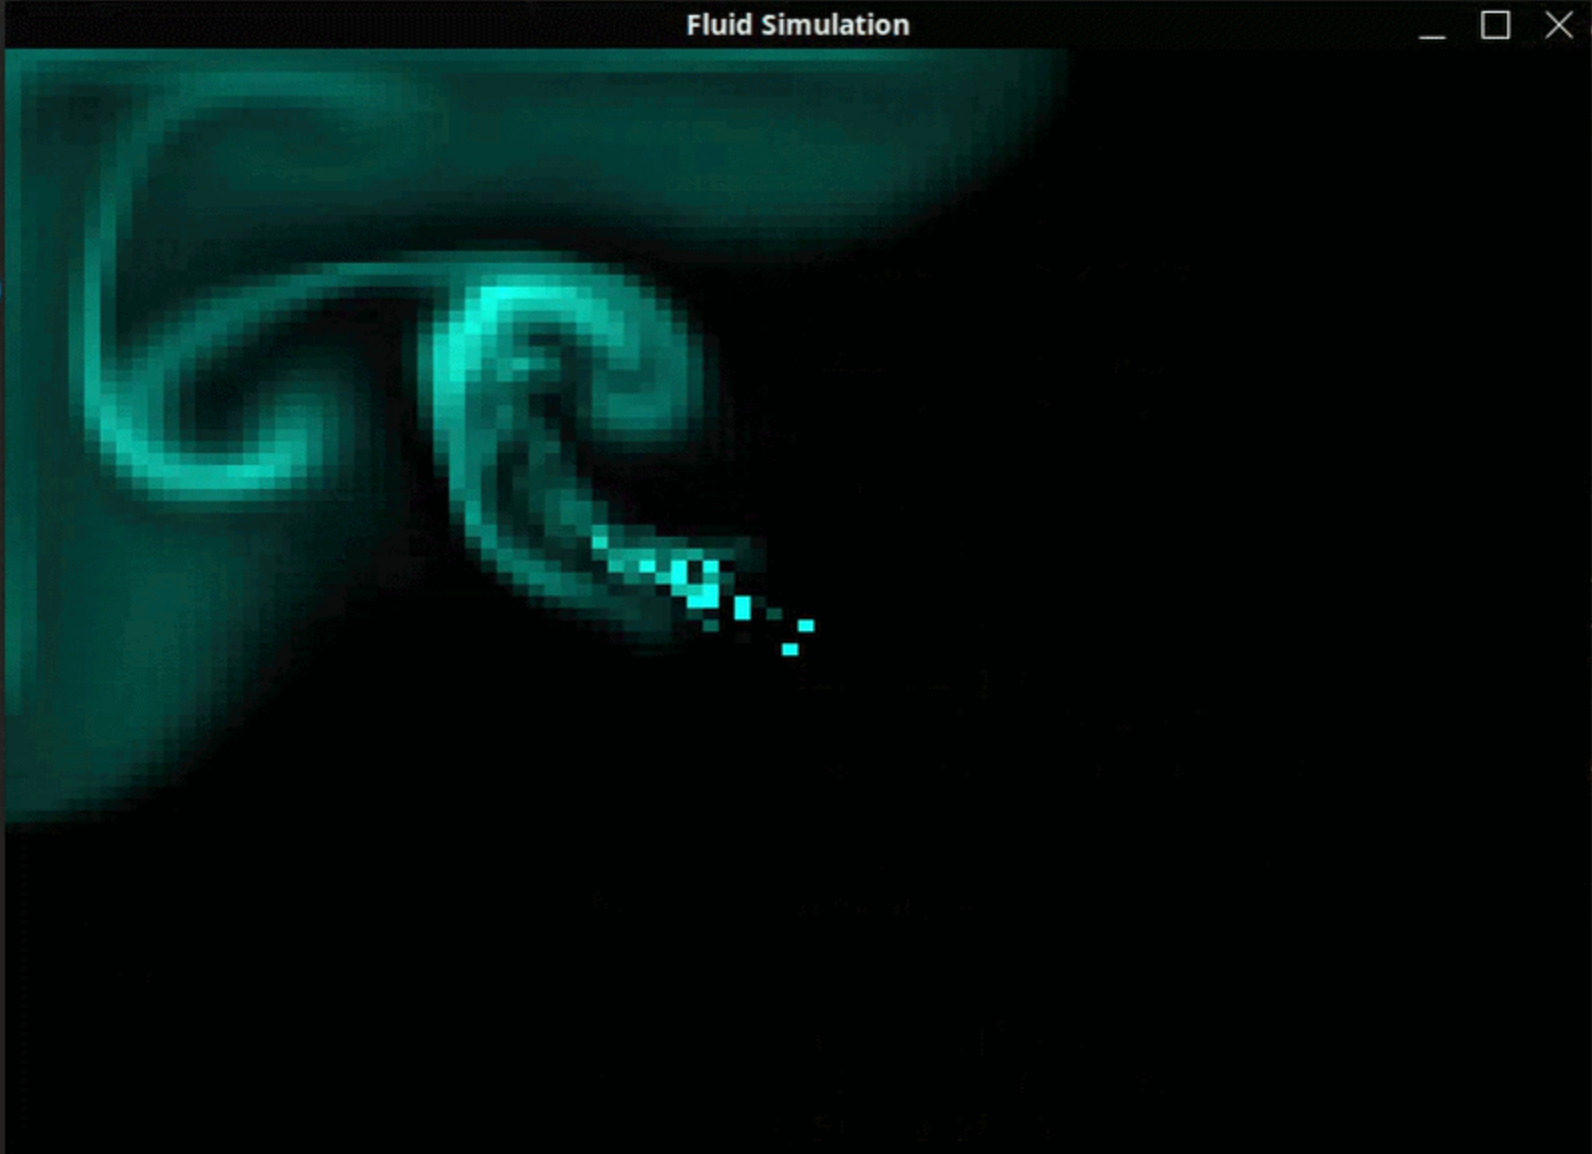
\includegraphics[width=0.45\textwidth]{PJ_proj/simulation_evol1.png}
        \caption{Deuxieme version : affichage d'un fluide.}
        \label{evolution2}
    \end{figure}

    \subsection*{Évolution 3 : ajout du panneau de paramètres (voir figure3)}
    {\color{green}Nous avons ensuite ajouté un panneau de paramètres en utilisant la bibliothéque ImGui.
    Ce panneau nous permet de modifier en temps réel, lors de la simulation, différents paramètres tels que la densité,
    la couleur ou encore la direction du fluide. Les valeurs saisies par l'utilisateur sont envoyées au module de simulation
    qui met à jour la grille. Notons que ce panneau peut s'enlever et se remettre en pressant la touche "h".}

    \begin{figure}[H]
        \centering
        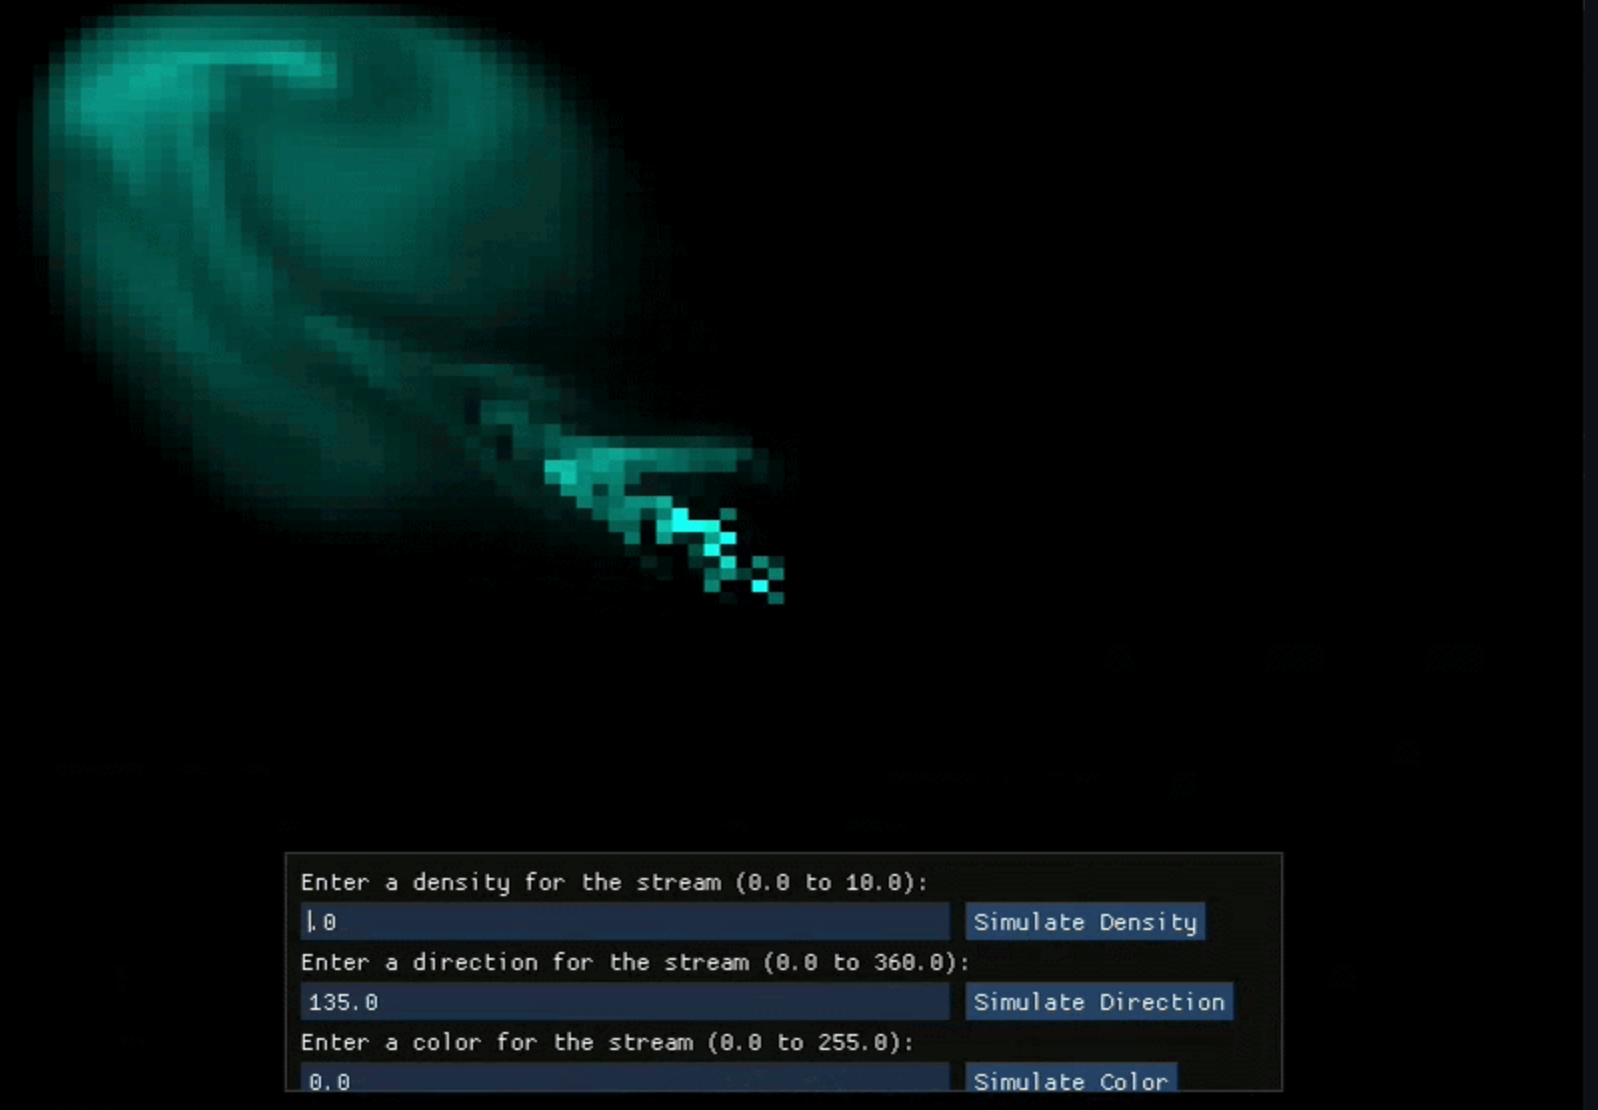
\includegraphics[width=0.45\textwidth]{PJ_proj/simulation_evol2.png}
        \caption{Troisième version : ajout d'un panneau de paramètres.}
        \label{evolution3}
    \end{figure}


    \subsection*{Évolution 4 : gestion des obstacles }
    {\color{green}Enfin nous avons étoffé notre simulation en ajoutant des obstacles. 
    Nous avons donc rajouté au panneau de paramètres les différents outils pour contrôler ceux-ci. 
    En effet, l'utilisateur peut activer ou désactiver les obstacles et changer leur forme, nous pouvons également
    rajouter plusieurs obstacles. Lors de la simulation,
    nous pouvons les déplacer avec le curseur de notre souris. Nous avons également implémenté deux modes d'injection
    du fluide : un point ou une ligne qui modifient le comportement du fluide. Par
    la même occasion nous avons rajouté un mode d'affichage 
    représentant la chaleur du fluide, l'utilisateur choisi sur le panneau de paramètres si le fluide
    sort chaud ou froid (rouge ou bleu). }

    \begin{figure}[H]
        \centering
        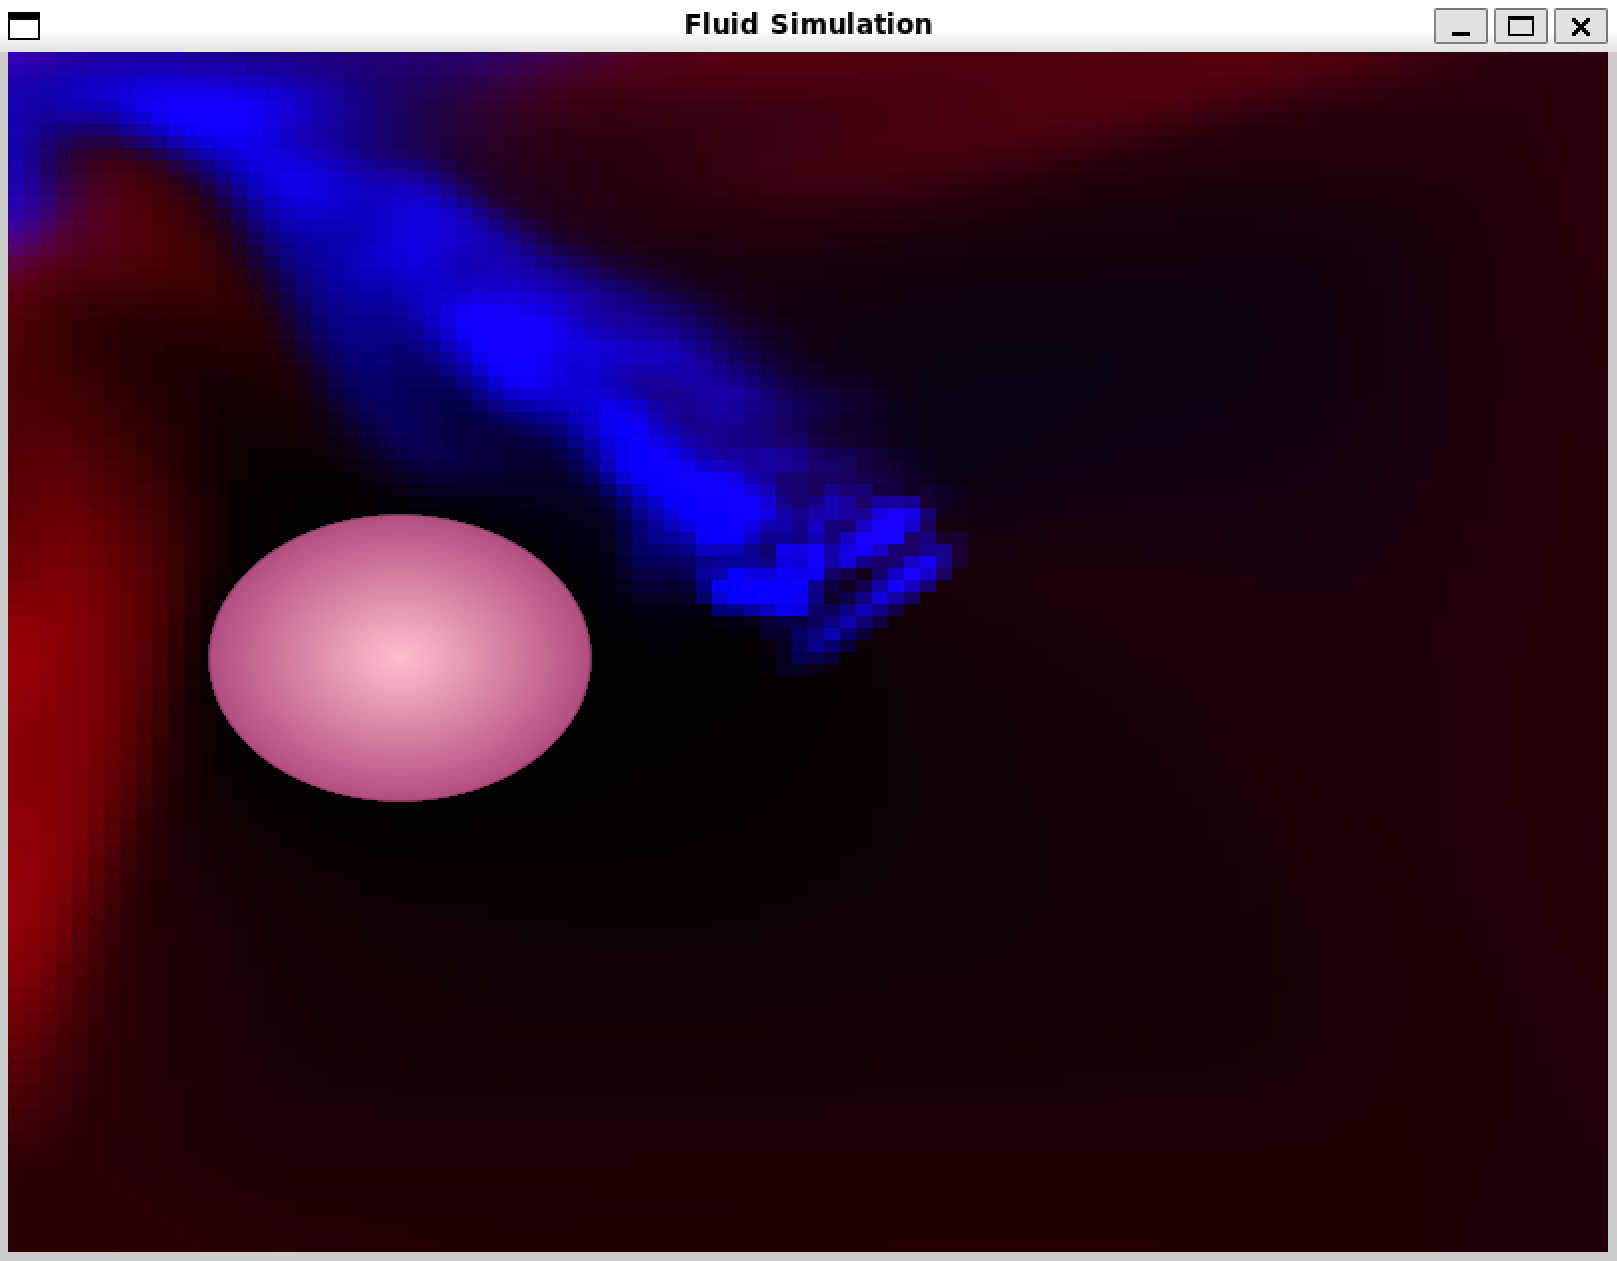
\includegraphics[width=0.45\textwidth]{PJ_proj/simulation_evol3.png}
        \caption{Quatrième version : ajout d'un obstacle.}
        \label{evolution4}
    \end{figure}





\item Présenter les principaux modules du logiciel développé dans le cadre du projet. Utiliser le langage UML pour la modélisation : donner le diagramme de cas d'utilisation et le diagramme des classes.
\begin{itemize}
    \item diagramme UML (cellules, grille, etc)
    \item PARTIE A : terminé, bien implémenté
    \item grille de départ (axel) (description des modules dans l'état actuel/final du projet)
    \item obstacle (satine)\\
            {\color{WildStrawberry} Dans un premier temps, nous avons implementer la creation 
            d'un unique obstacle en modifiant pour cela la fonction de gestion des dords ainsi que le main.
            nous pouvions egalement afficher ou non cette obstacle a l'aide d'un bouton on/off.
            suite a cela nous avons rendu cette obstacle interactif en offrant a l'utilisateur la 
            possibilite de le deplacer a l'aide du curseur de la souris.\\
            Nous avons ensuite étoffé notre simulation en ajoutant la possibilité d'avoir plusieurs obstacles,
            mais egalement celle de choisir la forme entre un 
            coeur, un cercle et une etoile. Pour cela, les obstacle ont ete 
            mis dans une liste (coordonnée,rayon,forme) afin de les rendre facilement reconnaissable et selectionnable.
            (ainsi, le premier obstacle de la liste est celui qui est prioritaire pour etre deplacer et le dernier obstaclede la liste es le
            premier retirer).on peut ainsi choisir le nombres d'obstacle grace u a un boutons +/- devant chaque forme possible.
            Pour chaque forme d'obstacle, nous avons dut
            crer une fonction qui genere les bords de la forme en question
            et une fonction pour l'affichage (afin d'avoir un obstacle colorer).
            Ainsi, chaque obstacle peuvent etre deplacer independament les uns des autres.
            Pour une bonne gestion des bords, il a fallut crer une fonction obstacleNormal qui
            permet de calculer la normale a l'obstacle en fonction de sa forme et de sa position, 
            ce qui nous a permis d'avoir une bonne gestion des bords du fluide et une bonne direction
            pour les fluides. Cette fonction gere la vitesse d'impacte et de rebond du fluides
            en fonction de la normale a l'obstacle, rendant le renvoi du fluide plus réaliste.

            } 
    \begin{figure}[H]
        \centering
        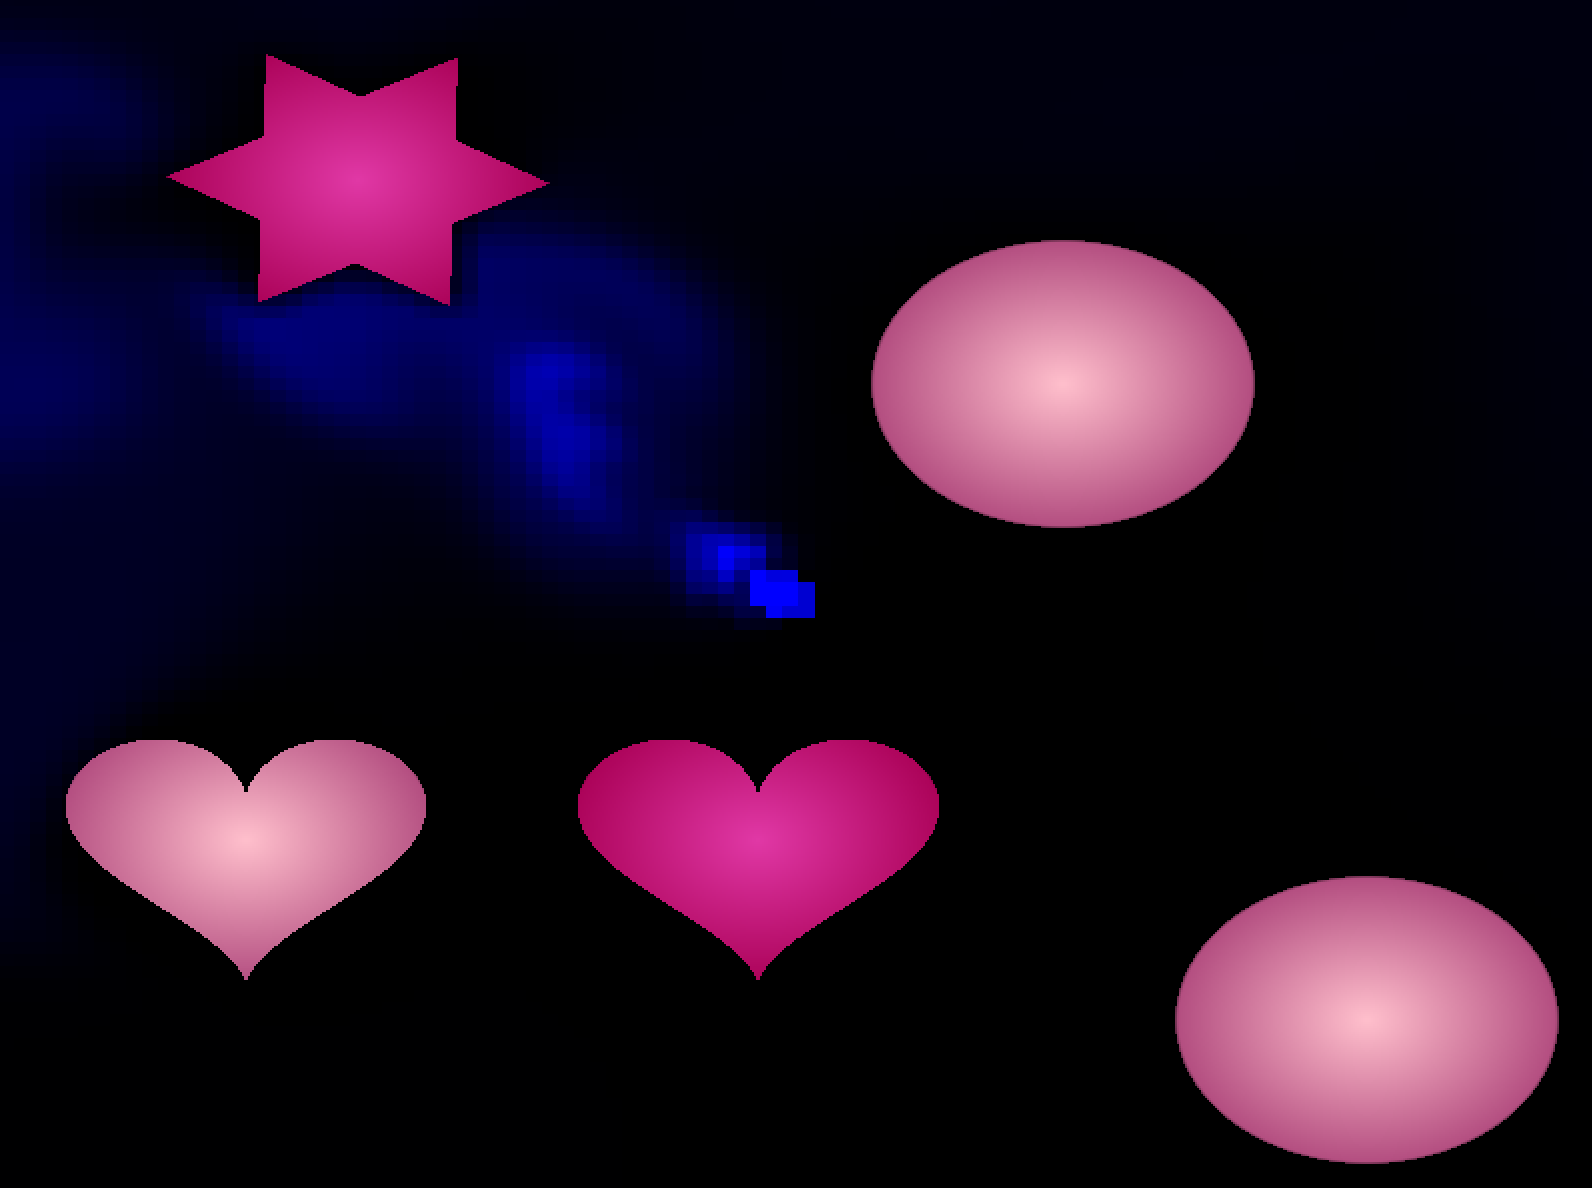
\includegraphics[width=0.45\textwidth]{PJ_proj/tout_les_obstacles.png}
        \caption{Ajout de plusieurs obstacles.}
        \label{evolution4}
    \end{figure}
    \item chaleur (saurane)
    \item point ou ligne (gaelle)
    \item calcul d'une simulation, le fluide, physique 
    \item PARTIE B : pas terminé
    \item bluetooth, lagrangien, musique, etc
\end{itemize}

\item Décrire les fonctionnalités de l'interface graphique implémentée (champs de simulation, bouton, affichage de l'obstacle).
\begin{itemize}
    \item description des boutons et des interactions possibles
\end{itemize}

\item Décrire le format des données en entrée ou encore les conventions utilisées pour les entrées de vos programmes.(représentation du fluide, grille, stackage des paramètres)
\begin{itemize}
    \item fluide stocké dans une grille
    \item grille composée de cellules
    \item cellules contiennent les paramètres de la simulation (densité, chaleur, vitesse)
    \item expliquer ce que représentent ces paramètres

\end{itemize}
\item Statistiques du projet

{\color{red}En termes de statistiques, notre projet est composé de certaines classes principales : Cellule, Grille, Obstacle, etc. Il est composé de 22 fichiers (cpp et h), 
et contient plus de 2000 lignes de code.
Le projet est organisé en plusieurs modules, tels que le module de gestion des obstacles, le module de gestion de la chaleur, etc.
}


\end{enumerate}

\section{Algorithmes et Structures de Données}
\emph{2 à 3 pages}

\begin{enumerate}%pour faire une liste numérotée
\item Présenter les principaux algorithmes implémentés. En illustrer le fonctionnement avec des exemples. Attention : il s'agit ici de choisir 1 ou 2 algorithmes intéressants, et non pas de présenter tous les algorithmes implémentés.

    \subsection*{L'Advection}
    \subsection*{La Diffusion}
    {\color{WildStrawberry}Comme l'advection, la diffusion est un processus 
    physique qui décrit la propagation d'une substance 
    (comme la chaleur ou la densité) à travers un fluide.
    On peut modeliser la diffusion à l'aide de l'équation de diffusion suivante:
        \begin{equation}
            x_{i,j}^{t+1} = x_{i,j}^{t} + \alpha \left( 
            (x_{i+1,j}^{t} - 2x_{i,j}^{t} + x_{i-1,j}^{t}) 
            + (x_{i,j+1}^{t} - 2x_{i,j}^{t} + x_{i,j-1}^{t}) 
        \right)
    \end{equation}
    Cette algorithme utilise la methode de resolution de l'equation
     de diffusion par relaxation de Gauss-Seidel, qui consiste à iterer sur chaque cellule de la 
     grille et à mettre à jour sa valeur en fonction des valeurs de ses voisins.
    }
    \subsection*{La Projection}
    {\color{red}Après avoir appliqué les algorithmes d'advection et de diffusion, l'algorithme de projection implémente la décomposition de Hodge. C'est un algorithme qui permet de rendre le champ de vitesse du fluide incompressible, 
    Cet algorithme force la vitesse à être conservatrice de masse, c'est à dire que le fluide ne peut pas être créé ou détruit. C'est une
    propriété importante pour une simulation réaliste. Visuellement, la projection force l'écoulement à avoir de meilleures courbes, et évite les écoulements en ligne droite. \\
    L'algorithme de projection est composé de 3 étapes :
    \begin{itemize}
        \item calcul de la divergence : pour chaque cllule de la grille, on évalue la divergence discrète :
        \begin{equation}
            {div}_{i,j} = -\frac{h}{2}left(u_{i+1,j} - u_{i-1,j}ight) + left(v_{i,j+1} - v_{i,j-1}ight)
        \end{equation}
        où $h = 1/N$ est la taille d'une cellule de la grille, et $u$ et $v$ sont les composantes de la vitesse du fluide.
        \item résolution de l'équation de Poisson : \\
        On résout itérativement l'équation $\nabla^2 p = div$ par 20 itérations de relaxation de Gauss-Seidel, où $p$ est un champ de pression :
        \begin{equation}
            p_{i,j}^{(k+1)} = \frac{1}{4}left({div}_{i,j} + p_{i+1,j}^{(k)} + p_{i-1,j}^{(k)} + p_{i,j+1}^{(k)} + p_{i,j-1}^{(k)} - div_{i,j}ight)
        \end{equation}
        On réutilisa exactement le code de la diffusion pour assurer la cohérence du code et éviter les redondances.
        \item correction du champ de vitesse : \\
        pour chaque cellule de la grille, on corrige la vitesse en soustrayant le gradient du champ de pression :
        \begin{equation}
            mathbf{u}'_{i,j} = \mathbf{u}_{i,j} - \frac{1}{2h} \begin{pmatrix} p_{i+1,j} - p_{i-1,j} \end{pmatrix}
        \end{equation}
    \end{itemize}}
    
\item Évaluer la complexité théorique en temps des algorithmes présentés
    \begin{itemize}
        \item complexité globale de update\_simulation
    \end{itemize}

\end{enumerate}

\section{Analyse des résultats }
\emph{2 à 4 pages}
L'analyse expérimentale sera faites dans cette section.   Elle sera plus ou moins importante dans votre projet comme pour les deux points précédent, cette section devra donc être développée en conséquence.

\begin{enumerate}%pour faire une liste numérotée

\item Illustrer les performances ainsi que l'efficacité du logiciel implémenté à l'aide de graphiques.
\begin{itemize}
\item calcul de complexités en fonction de la taille de la grille, etc (plot sur python), nombre d'obstacles, étape d'avection/relaxation (changer les paramètres et comparer)
\end{itemize}

\item Analyser (et comparer, si plusieurs) les performances des solutions implémentées.
\begin{itemize}
\item eulerien vs lagrangien (uniquement eulerien a été implémenté)
\item analyser les performances visuelles en fonction du nombre d'obstacles, densité, etc (mettre des screens)
\end{itemize}


\end{enumerate}

\section{Gestion du Projet}
\emph{ (1-2 pages)}
\begin{enumerate}%pour faire une liste numérotée
\item 	Présenter la gestion du projet et les documents de planification rédigés (par exemple, le diagramme de Gantt).
\begin{itemize}
    \item répartition des roles\\
    {\color{WildStrawberry}   Durant le project, nous avons dans un premier temps travailler ensemble
pour la mise en place de la grille de départet la creation du fluide
ainsi que pour l'affichage de celui ci. Une fois cette partie terminée, nous avons ensuite
 décidé de nous répartir les tâches pour être plus efficace.
 Ainsi, Gaelle a travailler sur les differents curseur avec Axel, Satine a
 travailler sur les obstacles, Axel à egalement travailler sur le bleetooth, et Saurane a travailler 
 sur la diffusion de la chaleur.}
 
    \item diagramme de gantt
    \item branches github, commits \\
    {\color{WildStrawberry} Pour la mise en place d'un travaille d'equipe
    optimale, nous aveons utilisé github. Lorsque nous travaillions ensemble, 
    nous nous placions sur la branche main afin que chacun puise acceder 
    a ce que les autres ont fait facilement, puis lorsque nous avons choisit 
    de nous repartir les taches nous nous sommes tous mis à
    travailler sur des braches differentes (Gaelle, Satine,Axel,Saurane)
    afin de pouvoir travailler et enregistrer notre travaille
    sans risquer de causer des conflits ou d'enreistrer quelque chose qui ne fonctionne pas.
    Une fois notre programme complet nous le metions alors sur le main afin que tous le monde puisse y acceder.}
\end{itemize}
\item	Discuter les changements majeurs effectués en cours de projet. 
\begin{itemize}
\item passage de la grille de départ à la nouvelle grille (pourquoi?)
\item la façon d'implémenter les obstacles a été modifiée quand on est passé de l'affichage d'uun obstacle à plusieurs, est-ce
    que ça a impacté les autres modules ? pourquoi? comment ?\\
    {\color{WildStrawberry} 
      Pour les creation d'obstacle, il a fallut dans un premier temps readapter la fonction
      qui delimiter les bord du fluides afin que celui ci prenne en compte l'object
      ce qui a crer de nombreux probleme (la disparition du fluide a travers l'obstacle ou la fuite du fluide a travers les bords).
      ou encore des probleme de dependance entre les diferents obstacles lorsque que nous avons voulu
      ajouter plusieurs obstacles mobile. De plus, l'implementation d'obstacle ayant une autre forme
      que la boule pose de nombreux probleme notamment dans la partie de delimitation du fluides ou encore dans la partie d'affichage.
      Pour resoudre ces probleme il a fallut revoir le code en changement la facon de voir 
      les obstacles mais également en les implementant de maniere differente.
      Ainsi, les obstacle ont ete ranger une une liste afin que le premier obstacle soit reconnaisable
      et ceux ci sont ainsi selectionner a partir du premier de la liste lorsqu'il fuat
      les afficher et c'est le dernier obstacles qui est effacer lorsque l'on desire e retirer un.
    }   

\item implémentation de la fenetre pour rentrer les paramètresuu
\end{itemize}
\end{enumerate}

\section{Bilan et Conclusions}

	Indiquer les fonctionnalités mises en œuvre par rapport au cahier des charges de départ, les points ouvertes.
	Les perspectives du projet décrivent ce que l’on pourrait ajouter, modifier, réécrire afin d’améliorer le projet. 

\begin{enumerate}
    \item Fonctionnalités rélisées qui étaient présentent dans le cahier des charges 
    \begin{itemize}
        \item interface graphique avec une fenetre d'affichage du fluide et des curseurs
        \item simulation du fluide en 2D
        \item possibilité d'agir sur le fluide avec des curseurs
        \item possibilité d'ajouter des obstacles
    \end{itemize}

    \item Fonctionnalités non rélisées qui étaient présentent dans le cahier des charges
    \begin{itemize}
        \item possibilité de controler le fluide à distance via un smartphone (bluetooth)
        \item intégrer un mode musique qui fait réagir de fluide en focntion du son
    \end{itemize}
\item Perspecvtives du projet pour la suite : ce qu'on aurait pu implémenter avec plus de temps.
\begin{itemize}
    \item lagrangien
    \item autres fonctionnalités possibles avec les obstacles, etc
\end{itemize}
\end{enumerate}

\begin{thebibliography}{9}
\bibitem{texbook}
Donald E. Knuth (1986) \emph{The \TeX{} Book}, Addison-Wesley Professional.

\bibitem{lamport94}
Leslie Lamport (1994) \emph{\LaTeX: a document preparation system}, Addison
Wesley, Massachusetts, 2nd ed.
\end{thebibliography}



\end{document}

